%!TEX program = xelatex

\documentclass[12pt, a4paper]{article}
\usepackage[utf8]{inputenc}
\usepackage[russian]{babel}
\usepackage{pscyr}

\usepackage{xifthen}
\usepackage{parskip}
\usepackage{hyperref}
\usepackage[top=0.7in, bottom=1in, left=0.6in, right=0.6in]{geometry}
\usepackage{setspace}

\usepackage{amsmath}
\usepackage{MnSymbol}
\usepackage{amsthm}
\usepackage{mathtools}

\usepackage{algorithm}
\usepackage[noend]{algpseudocode}



\linespread{1.2}
\setlength{\parskip}{0pt}

\renewcommand\familydefault{\sfdefault}


% Stuff related to homework specific documents
\newcounter{MyTaskCounter}
\newcounter{MyTaskSectionCounter}
\newcommand{\tasksection}[1]{
	\stepcounter{MyTaskSectionCounter}
	\setcounter{MyTaskCounter}{0}
	\ifthenelse{\equal{#1}{}}{}{
	{\hfill\\[0.2in] \Large \textbf{\theMyTaskSectionCounter \enspace #1} \hfill\\[0.1in]}}
}

\newcommand{\task}[1]{
	\stepcounter{MyTaskCounter}
	\hfill\\[0.1in]
	\ifthenelse{\equal{\theMyTaskSectionCounter}{0}}{
	   \textbf{\large Задача №\theMyTaskCounter}
	}{
	   \textbf{\large Задача №\theMyTaskSectionCounter.\theMyTaskCounter}
	}
	\ifthenelse{\equal{#1}{}}{}{{\normalsize (#1)}}
	\hfill\\[0.05in]
}

% Math and algorithms

\makeatletter
\renewcommand{\ALG@name}{Алгоритм}
\renewcommand{\listalgorithmname}{Список алгроитмов}

\newenvironment{procedure}[1]
  {\renewcommand*{\ALG@name}{Процедура}
  \algorithm\renewcommand{\thealgorithm}{\thechapter.\arabic{algorithm} #1}}
  {\endalgorithm}

\makeatother

\algrenewcommand\algorithmicrequire{\textbf{Вход:}}
\algrenewcommand\algorithmicensure{\textbf{Выход:}}
\algnewcommand\True{\textbf{true}\space}
\algnewcommand\False{\textbf{false}\space}
\algnewcommand\And{\textbf{and}\space}

\newcommand{\xfor}[3]{#1 \textbf{from} #2 \textbf{to} #3}
\newcommand{\xassign}[2]{\State #1 $\leftarrow$ #2}
\newcommand{\xstate}[1]{\State #1}
\newcommand{\xreturn}[1]{\xstate{\textbf{return} #1}}

\DeclarePairedDelimiter\ceil{\lceil}{\rceil}
\DeclarePairedDelimiter\floor{\lfloor}{\rfloor}

\newcommand{\bigO}[1]{\mathcal{O}\left(#1\right)}


\title{Формальные языки. Домашнее задание №4}
\author{Горбунов Егор Алексеевич}

\begin{document}
\maketitle

\begin{task}[1]
	Преобразовать в нормальную форму Хомского однозначную грамматику арифметических выражений, найти реализацию алгоритма CYK, запустить ее на полученной грамматике, трех различных корректных входах и трех некорректных, визуализировать полученные деревья вывода и записать сообщения об ошибках (прислать результаты работы парсера в pdf).
	\begin{align*}
		E &\rightarrow E + T\ |\ T \\
		T &\rightarrow T * P\ |\ P \\
		P &\rightarrow (E)\ |\ n
	\end{align*}
\end{task}
\begin{solution}
Грамматика у нас такая:
	\begin{align*}
		\Sigma &= \xbrace{+, *, (, ), n} \\
		N &= \xbrace{E, T, P}\\
		S &= E
	\end{align*}
$\varepsilon$-продукций в грамматике нет, а также нетрудно видеть, что абсолютно все символы грамматики достижимые и порождающие. 

Найдём все цепные пары индуктивно:
\[
	\begin{array}{l}
		(E, E)\\ (T, T)\\ (P, P)
	\end{array}
	\Rightarrow
	\begin{array}{l}
		(E, E)\\ (E, T)\\ (T, T)\\ (T, P)\\ (P, P)  
	\end{array}
	\Rightarrow
	\begin{array}{l}
		(E, E)\\ (E, T)\\ (E, P)\\ (T, T)\\ (T, P)\\ (P, P)\\  
	\end{array}
\]
Теперь удалим цепные пары и добавим нужные продукции в грамматику:
	\begin{align*}
		E &\rightarrow E + T\ |\ T * P\ |\ (E)\ |\ n\\
		T &\rightarrow T * P\ |\ (E)\ |\ n \\
		P &\rightarrow (E)\ |\ n
	\end{align*}
Теперь приведём к нормальной форме Хомского. Для начала избавимся от терминалов в правых частях продукций, длины больше 1:
	\begin{align*}
		L &\rightarrow (\\
		R &\rightarrow )\\
		X &\rightarrow *\\
		O &\rightarrow +\\
		E &\rightarrow E\ O\ T\ |\ T\ X\ P\ |\ L\ E\ R\ |\ n\\
		T &\rightarrow T\ X\ P\ |\ L\ E\ R\ |\ n \\
		P &\rightarrow L\ E\ R\ |\ n 
	\end{align*}
И разобьём наконец слишком длинные правила:
	\begin{align*}
		L &\rightarrow (\\
		R &\rightarrow )\\
		X &\rightarrow *\\
		O &\rightarrow +\\
		E &\rightarrow E\ D\ |\ T\ M\ |\ L\ C\ |\ n\\
		T &\rightarrow T\ M\ |\ L\ C\ |\ n \\
		P &\rightarrow L\ C\ |\ n\\
		D &\rightarrow O\ T\\
		M &\rightarrow X\ P\\
		C &\rightarrow E\ R\\
	\end{align*}
\end{solution}

Ниже изображены деревья (в силу особенностей \texttt{JFLAP} было добавлено правило $S \rightarrow E$ и круглые скобки $()$ заменены на квадратные $[]$).

\begin{figure}[ht!]
\centering
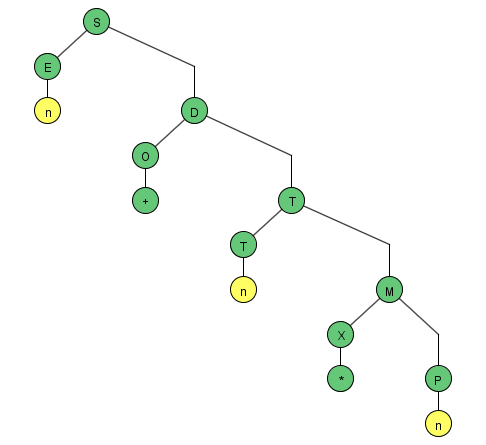
\includegraphics[scale=0.5]{t1.png}
\caption{Дерево выражения $n+n*n$}
\end{figure}

\begin{figure}[ht!]
\centering
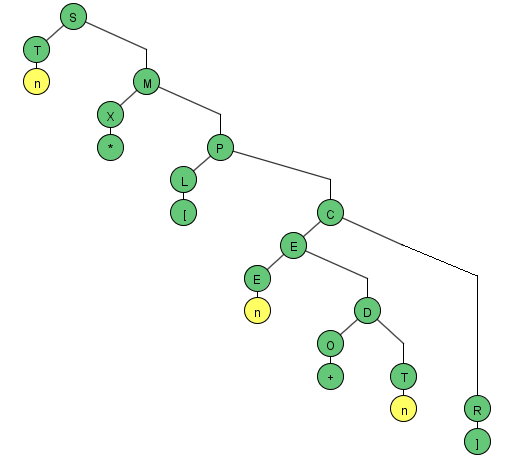
\includegraphics[scale=0.5]{t2.png}
\caption{Дерево выражения $n*[n+n]$}
\end{figure}

\begin{figure}[ht!]
\centering
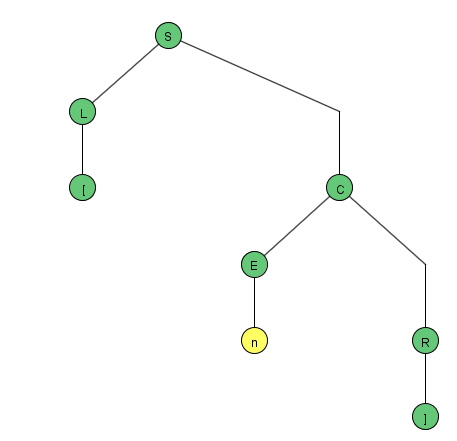
\includegraphics[scale=0.5]{t3.png}
\caption{Дерево выражения $[n]$}
\end{figure}

Все парсеры, которые я пробовал, не выдают информации об ошибке при неправильных вводах, поэтому картинки с <<недостроенными>> деревьями не прикреплены. Но ясно, что это были бы деревья, без верхушки :)

\end{document}